% Background Chapter

\chapter{Literature review} % Main chapter title
\label{ch1}

\section{What are Volatile Organic Compounds (VOCs)?}
\label{ch1:sec:what_are_vocs}
  Organic compounds are members of a large class of chemicals whose molecules contain carbon, with the exception of a few compounds such as carbides, carbonates (CO$_3$), and simple oxides of carbon and cyanides.
  Organic compounds can be categorised based on their vapour pressure, which is the tendency of a liquid or solid to vaporise.
  Compounds with high vapour pressures at standard temperature are classed as volatile, and have a felicity to evaporate at low temperatures.
  
  Atmospheric organic compounds are legion and differ by orders of magnitude with respect to their fundamental properties, such as volatility, reactivity, and cloud droplet formation propensity.
  VOCs have vapour pressure greater than $10^{-5}$~atm, and are mostly generated naturally by plants, which emit around 1000~Tg per year \citep{Guenther1995, Glasius2016}.
  Due to their high volatility these compounds are generally seen in the gas phase.
  Organic compounds with a lower volatility are classed as semi-volatile (SVOCs: vapour pressure between $10^{-5}$ and $10^{-11}$~atm) are seen in both gas and particle phase depending on temperature and pressure.
  Organic compounds with even lower vapour pressure are generally found in the particle phase in aerosol particulate matter \citep{Glasius2016}.

  Understanding the drivers of trends in biogenic volatile organic compound emissions (BVOCs) is needed in order to estimate future carbon fluxes, changes in the water cycle, air quality, and other climate responses \citep{Yue2015}.

  TODO read and reference \citep{Franco2015} 
  
%----------------------------------------------------------------------------------------
%	SECTION 1
%----------------------------------------------------------------------------------------
\section{Natural gas and aerosol emissions in Australia}
\label{ch1:sec:emissions}

  \subsection{Australia}

    Australia is largely covered by environments which are not heavily influenced by human activity.
    These environments are sources of naturally released trace gases which make up less than 1\% of earth's atmosphere.
    Naturally occurring trace gases in the atmosphere can have a large impact on living conditions.
    They react in complex ways with other elements (anthropogenic and natural), as well as affecting various ecosystems upon which life depends.
    Natural emissions affect surface pollution levels and can alter the radiative and particulate matter distribution of the atmosphere with harmful results.
    For example, ozone in the lower atmosphere is a serious hazard that causes health problems \citep{Hsieh2013}, damages agricultural crops worth billions of dollars \citep{Avnery2011}, and increases the rate of climate warming \citep{IPCC_2013_chap8}.
    Particulate matter in the atmosphere is also a major problem, causing an estimated 2-3 million deaths annually \citep{Hoek2013, Krewski2009, Silva2013, Lelieveld2015}.

    The Australian outback includes extremely large and diverse environments.
    Much of the landscape outside of urban areas is undeveloped and sparsely inhabited.
    In Australia most long term air quality measurements are performed in or near large cities.
    However, estimates of atmospheric gas and particulate densities, and their distributions over much of the continent are uncertain and lack in-situ measurements.
    %For instance the Total Carbon Column Observing Network (TCCON) has sites at Darwin and Wollongong, and the Aerosols Robotic Network (AERONET) 

  \subsection{Satellite Measurements}

    Natural emissions from areas with little anthropogenic influence and no ground based measurements characterise the majority of Australian land mass \citep{VanDerA2008}.
    One source of information which covers the entirety of Australia is remote sensing performed by instruments on satellites which overpass daily recording reflected solar (and emitted terrestrial) radiation.
    These can be used to quantify the abundance of several chemical species as well as estimate their distribution in vertical columns over the land.

    The existence of satellite data covering remote areas provides an opportunity to develop more robust models of global climate and chemistry.
    Understanding of emissions from these areas is necessary to inform national policy on air pollution levels.
    Satellite data allow us to verify large scale model estimates of natural emissions.
    These measurements can be used to improve models, which are then able to predict harmful and costly events.
    
    While satellite data is effective at covering huge areas (the entire earth) it only exists at a particular time of day, is subject to cloud cover, and generally does not have fine horizontal or vertical resolution.
    Concentrations retrieved from satellite have large uncertainties, which arise due to several factors which arise in the process of transforming spectra to total column measurements, as well as instrument degradation (satellite instruments are hard to tinker with once they are launched).
    
    There are two types of error, arguably the worst of the two is systematic error (or bias) which normally indicates a problem in calculation or instrumentation.
    If the systematic error is known, it can be corrected for by either offsetting data in the opposite direction, or else fixing the cause.
    A proper fix can only be performed if the sources of error are known and there is a way of correcting or bypassing it.
    Random error is the other type (often reported as some function of a dataset's variance or else uncertainty), and this can be reduced through averaging either spatially or temporally. 
    By taking the average of several measurements, any random error can be reduced by a factor of one over the square root of the number of measurements.
    This is done frequently for the relatively highly uncertain satellite measurements of trace gases (which are often near to the detection limit over much of the globe).
    For example: \citet{Vigouroux2009} reduce the measurement uncertainty (in SCIAMACHY HCHO columns) by at least a factor of 4 through averaging daily over roughly 500km around Saint-Denis, and only using days with at least 20 good measurements.

%----------------------------------------------------------------------------------------
%	Ozone Section
%----------------------------------------------------------------------------------------
\section{Ozone}
\label{ch1:sec:Ozone}
TODO: Start this section!
  \subsection{Basics}
    
    
  \subsection{Sources and sinks}
  
  \subsection{Measurements}
  TODO: Include ozone hole treaty and things put in place for that
%----------------------------------------------------------------------------------------
%	HCHO Section
%----------------------------------------------------------------------------------------
\section{Formaldehyde(HCHO)}
\label{ch1:sec:HCHO}
  
  \subsection{Basics}
    HCHO, aka methanal, methyl aldehyde, and methylene oxide is of the aldehyde family.
    HCHO is an OVOC which is toxic, allergenic, and a potential carcinogen. 
    It is dangerous at low levels, with WHO guidelines for prolonged exposure at 80ppb.
    
    HCHO is used as an adhesive in plywood and carpeting and also used in the creation of paints and wallpapers.
    Emissions in enclosed spaces can build up to dangerous levels, especially if new furnishings are installed \citep{Davenport2015}.
    One common way to detect and measure HCHO is through the DOAS technique, which takes advantage of the optically thin nature of HCHO in order to linearise the differential determined from the Beer-Lambert intensity law.
    This method works for both in the home HCHO detection and global measurements from in-situ and remote sensing instruments \citep{Guenther1995, Abad2015,Davenport2015}.
    
  \subsection{Sources and sinks}
    In the atmosphere HCHO is primarily produced through the oxidation of methane (CH$_4$) by the hydroxyl radical (OH).
    Within the continental boundary layer, the major source of HCHO enhancement is VOC emissions reacting with OH radicals in the presence of NO$_X$ \citep{Wagner2002, Millet2006}.
    
    HCHO follows two major reactions with the hydroxyl radical (OH), producing hydroperoxyl radicals (HO$_2$), and leading to a change in the atmospheric oxidative capacity \citep{Crutzen1999, Wagner2002}.
    The other main sink is photolysis, (todo: levy 1972 read abstract and cite), combined with the OH reactions leads to a daytime lifetime of a few hours (todo: read abstract and cite atkinson 2000) \citep{Millet2006}.
    The other major sinks are wet and dry deposition.
    
    In the past, HCHO levels were underestimated by models, often with large discrepancies, due to the poor understanding of methyl peroxy radical (CH$_3$OO) chemistry \citep{Wagner2002}.
    
  \subsection{Measurements}
    There are a few ways to measure HCHO, including FTIR and MAX-DOAS. 
    As a trace gas HCHO interferes with light over a few wavelength bands, which allows instruments to detect concentrations along a path between a sensor and a known light source like a lamp or the sun.
    Figure \ref{ch1:fig:HCHOSpectrum} shows the interference spectrum of HCHO as well as a typical band used to examine interference in the DOAS technique.
    One difficulty is that this interference is relatively small (HCHO is optically thin) and other compounds absorb light at similar wavelengths \citep{Davenport2015}.
    
    \begin{figure}
      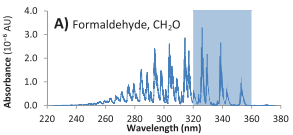
\includegraphics{Figures/HCHO/HCHOAbsorbanceDavenport.png}
      \caption{ HCHO spectrum, with a typical band of wavelengths used for DOAS path measurements.
	This is a portion of an image from \citet{Davenport2015}.}
      \label{ch1:fig:HCHOSpectrum}
    \end{figure}
    
    Other measurement techniques include chromatographic and fluorimetric methods, both of which differ widely from eachother and the spectroscopic method TODO: read \citep{Hak2005}).
    This resulted in HCHO not having a consistent network for global measurements like those for GHGs or Ozone \citep{FortemsCheiney2012}.
    
  \subsection{Relationship with glyoxyl and isoprene}
    Glyoxyl (CHOCHO) is important to us as it shares many properties with HCHO, and may provide additional information in determining isoprene emissions.
    Glyoxyl is another product of VOC oxidation in the atmosphere, with isoprene being the main source globally.
    Isoprene has been used to estimate isoprene emissions (see section \ref{ch1:sec:IsopFromHCHO}) but many uncertainties exist.
    One of these uncertainties is the yield of HCHO from isoprene, especially in low NO$_X$ environments.
    Glyoxyl could prove complementary to HCHO in constraining isoprene emissions (TODO: Read and cite Vrekoussis2009,2010, Chan Miller 2014, Alvarado 2014).
    
    Under high NO$_X$ conditions, glyoxyl forms rapidly, similarly to HCHO.
    However, glyoxyl also forms in low NO$_X$ environments both slowly (through isoprene epoxydiols), and rapidly (through di-hydroperoxide dicarbonyl compound photolysation (todo: read abstract and cite crounse(Autoxidation of Organic Compounds in the Atmosphere) 2013).
    This process is similar to the proposed mechanisms for hydroperoxyaldehydes by \citet{Peeters2014} and carbonyl nitrates (todo: read and cite M$\:{u}$ller 2014).
    
  \subsection{Satellite measurements}
    Satellite measurements of HCHO are relatively uncertain, however this can be improved by averaging over larger grid boxes or longer time scales.
    an example of this can be seen in (TODO: read/cite dufour2009), where monthly averaging is used to decrease the measurements uncertainty.
    HCHO in Europe is low; near the detection limit of satellite measurements, however taking monthly averages allows enough certainty that useful inversions can be determined to estimate the sources of the HCHO (TODO: read and citep{Dufour2009}).
    
    For many places the tropospheric column HCHO measured by satellite is biased low, \citet{Zhu2016} examine six available satellite datasets and show a bias of 20 - 51\% over south east USA when compared against a campaign of aircraft observations (SEAC$^4$RS).
    \citet{DeSmedt2015} also found a low bias from 20 - 40\% when comparing OMI and GOME2 observations against ground based vertical profiles, and \citet{Barkley2013} determine OMI to be 37\% low compared with aircraft measurements over Guyana.
    These bias can be corrected by improving the assumed apriori HCHO profiles which are used to calculate the AMFs of the satellite columns.
    
    The OMI measurements used in this research are recalculated using an updated estimate of HCHO profiles and validated against Wollongong total column measurements. 
    Similar to validation performed by other studies TODO: cite and exemplify a few studies ie: \citet{Zhu2016,Marais2015,Palmer2003} 
    
    Uncertainty in the OMI satellite instrument is calculated by the Smithsonian Astrophysical Observatory (SAO) group using the uncertainty in backscattered radiation retrievals \citep{Abad2015,Abad2016}.
    Another method of calculating the uncertainty is used by the Belgian Institute for Space Aeronomy (BIRA) group, who determine uncertainty from the standard deviation of HCHO over the remote pacific ocean (TODO: use both these methods for HCHO section)\citep{DeSmedt2012,DeSmedt2015}.
%----------------------------------------------------------------------------------------
%	Isoprene Section
%----------------------------------------------------------------------------------------
\section{Isoprene}
\label{ch1:sec:isoprene}

  \subsection{Basics}
    Isoprene, or 2-methylbuta-1,3-diene, is a Volatile Organic Compound (VOC) and has chemical formula of C$_5$H$_8$. 
    Isoprene effects NO$_X$ and HO$_Y$ cycling, and in the presence of NO$_X$, forms tropospheric ozone and SOAs \citep{Wagner2002, Millet2006}.
    Bottom up inventories of VOCs remain largely uncertain due to extensive extrapolation over plant functional types, changing land cover, and parameterised environmental stressors (todo: read and \citep{Guenther2000}).
    

  \subsection{Sources and Sinks}
    Methane and isoprene each comprise around a third of the yearly global total emission of VOCs.
    However, methane is relatively long lived (years) and is well mixed in the atmosphere while isoprene levels are very volatile and spatially diverse due to a life time of around an hour.
    Estimates put global isoprene emission at roughly 600 Tg yr$^{-1}$, emitted mostly during the day.
    The major emitters are tropical broadleafs, eucalypts, and scrubs \citep{Guenther2006, Arneth2008, Niinemets2010, Monks2015}.

    Biogenic isoprene emissions are far greater than anthropogenic emissions of VOCs \citep{Guenther2006, Kefauver2014}. 
    The lack of accuracy in BVOC emissions estimates has a large effect on determining with confidence the sources and distribution of pollutants including ozone and organic aerosols.
    Accuracy in VOC measurements is important: it has been shown that even the diurnal pattern of isoprene emissions has an effect on modelling ground level ozone \citep{Hewitt_2011,Fan_2004}.
    These uncertainties could explain why models of HCHO over Australia are poor at reproducing satellite measurements \citep{Stavrakou2009}.

    \citet{Guenther2006} estimates that the Australian outback is among the world's strongest isoprene emitters with forests in SE Australia having emission factors greater than 16 mg m$^{-2}$ h$^{-1}$ (see figure \ref{ch1:fig:meganisoprene}).
    These emissions factor estimates are not well verified as there is little coverage of isoprene (or other BVOC) emissions measurements over Australia.
    However, comprehensive coverage of one of the products of isoprene chemistry in the atmosphere over Australia exists in the form of satellite measurements.
    
    It is important to note that many estimates of isoprene emission are based on a few algorithms of isoprene emission which can depend greatly on input parameters \citep{Niinemets2010}.
    \citet{Yue2015} has shown that this is still a problem by looking at land carbon fluxes and modelling the sensitivity to VOC emissions estimates using two independent models of VOC emission.
    One model is photosynthesis based and estimates isoprene emissions based, while the other (MEGAN) uses the light and canopy temperature (Niinemets et al., 1999; Arneth et al., 2007; Unger et al., 2013).
    
    \begin{figure}
      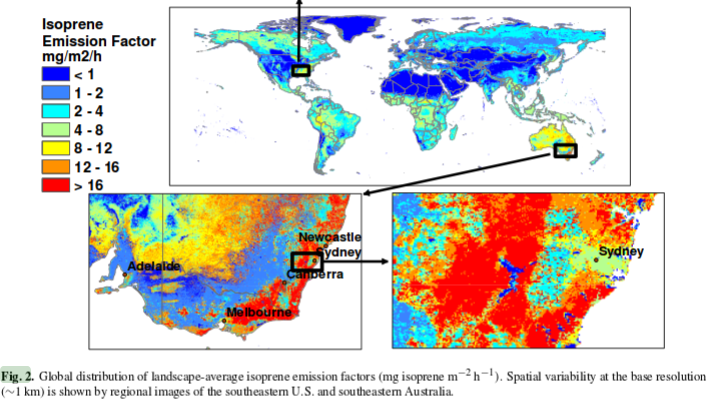
\includegraphics{Figures/MeganIsoprene1.png}
      \caption{ Part of a figure from \citet{Guenther2006} showing global isoprene emission factors. }
      \label{ch1:fig:meganisoprene}
    \end{figure}
    
  \subsection{Isoprene From HCHO}
    \label{ch1:sec:IsopFromHCHO}
    In the remote troposphere HCHO production is dominated by methane oxidation, while in the continental boundary layer (CBL) production is largely due to NMVOCs \citep{Abbot2003,Kefauver2014}.
    NMVOCs are alkanes, alkenes, aromatic hydrocarbons and isoprene.
    Isoprene is hard to measure directly due to its short lifetime and weak spectral absorption, instead formaldehyde is often used as a proxy \citep{Millet2006,Marais_2012,bauwens2013satellite,Kefauver2014,Bauwens2016}.
    Formaldehyde formed in the troposphere is mostly due to VOC (roughly one third each: methane, isoprene, others) oxidation. 
    We can model this oxidation process in order to work out how much VOC is present based on the total HCHO.
    This requires among other things an idea of which VOCs are present and their yeilds of HCHO.
    
    The method used to develop top-down isoprene inference using satellites was developed initially by \citet{Palmer2001,Palmer2003}. 
    Isoprene emissions fluxes were derived using the Global Ozone Monitoring Experiment (GOME) satellite instrument.
    Palmer's method improved biogenic isoprene emissions estimates (compared with in-situ measurements) over two available inventories: the U.S. EPA Biogenic Emssions Inventory System (BEIS2) and the Global Emissions Inventory Activity (GEIA).
    This showed an inversion technique which could be used to improve large scale emissions estimates without further expensive measurement campaigns.
    
    Satellites recording reflected solar spectra use Differential Optical Absorption Spectroscopy (DOAS) to measure various trace gases in the atmosphere, including formaldehyde. 
    Formaldehyde levels in the continental boundary layer are generally dominated by chemical formation due to VOC (largely isoprene) emissions \citep{Kefauver2014}.
    
    Satellites can be used to measure the seasonal and interannual variability of HCHO over Australia.
    These records can be compared with modeled estimates of HCHO and used as a proxy to estimate isoprene emissions.
    This has been done in North America \citep{Palmer2003, Millet2006}, South America, Africa, China, Europe, and recently globally \citep{FortemsCheiney2012, Bauwens2016}.
    Often these works use two forms of measurement such as satellite and aircraft data combined for validation \citep{Marais_2014}.
    
    Initially studies assumed a simple linear steady-state relationship between HCHO and it's precursors \citep{Palmer2003,Palmer2006,Millet2006}.
    This allowed a simple calculation of isoprene using the measured HCHO, with estimated reaction rates and yields.
    The methodology for calculating VOCs from HCHO is laid out in \citet{Palmer2003}, and takes into account the expected lifetime and reaction rates of the precursor VOCs and HCHO.
    Assuming HCHO is produced quickly from short-lived intermediates, and the column is at steady state:
    \begin{eqnarray*}
    VOC_i \overset{k_i}{\rightarrow} Y_i HCHO
    \end{eqnarray*}
    Where $Y_i$ is HCHO yield per C atom (a measure of how much HCHO will form per gram of C from a VOC within a system), and $k_i$ is the reaction rate.
    Then assuming a steady state of atmospheric HCHO ($\Omega$ molecules $cm^{-2}$) produced by oxidation of VOCs (VOC$_i$) and no horizontal transport:
    \begin{eqnarray*}
    \Omega = \frac{1}{k_{HCHO}} \sum_{i} Y_i E_i
    \end{eqnarray*}
    Where i indexes a chemical species, $k_{HCHO}$ is the HCHO loss rate due to OH and photolysis, Y$_i$ is the HCHO yield, and $E_i$ is emission fluxes ( C atoms $cm^{-2}s^{-1}$).
    
    
    Estimates of Y$_i$ can be attained from a model as shown in \citet{Millet2006}.
    This involves a reduced major axis (RMA) correllation calculation between modelled HCHO and isoprene columns, multiplied by their reaction rates (as a normalising factor).  
    In high NOx environments where HCHO has a lifetime on the order of 30 minutes, it can be used to map isoprene emissions with spatial resolution from 10-100 kms.
    Horizontal transport 'smears' the HCHO signal so that source location would need to be calculated using windspeeds and loss rates \citep{Palmer2001,Palmer2003}.
    For more details on this see section \ref{ch1:sec:smearing}.
    
    Another method of correcting isoprene emissions using observed HCHO total column involves a Bayesian inversion.
    In \citet{Curci2010}, a regional CTM (CHIMERE) simulates HCHO, which is compared against OMI observed HCHO and shown to be regionally biased.
    This is expected to be due to errors in MEGAN's natural isoprene emissions.
    The CHIMERE model is used to derive yields of HCHO from the various local VOCs and these yields are then used in estimating  local emissions.
    The Bayesian inversion is used to correct regionally biased biogenic isoprene emissions through determination of the emissions which more closely(to the observed HCHO) simulate HCHO.
    (TODO: summary of this bayesian method from Curci2010).
    \cite{Curci2010} uses CHIMERE as the forward model to determine the relationship between HCHO (y), isorene and reactive anthropogenic VOCs (\textbf{x}), using 
    \begin{equation}
        y=\mathbf{K}x + b + \epsilon
    \end{equation}$
    where b is the background HCHO determined from CHIMERE with desired emissions set to zero, and $\epsilon is (assumed independent) errors in measurements.
    K is the Jacobian matrix determined from CHIMERE representing the sensitivity of y to the state variable x.
    This K matrix is used in conjunction with error covariance in x to determine the Maxium A Posteriori (MAP) solution to give an optimal estimate of x ($\hat{x}$). 
    
    TODO: Read through this list of sources on the hcho to isop process : taken from Wolfe2015
    Such techniques have informed isoprene emission inventories in North America (Abbot et al., 2003; Millet et al., 2008, 2006; Palmer et al., 2006, \citep{Palmer2003}), South America (\citep{Barkley2013}, 2008), Europe (\citep{Curci2010}, Dufour et al., 2009), Africa (Marais et al., 2012), Asia (Fu et al., 2007; Stavrakou et al., 2014), and globally (Fortems-Cheiney et al., 2012; Shim et al., 2005; Stavrakou et al., 2009).
    
    More recently, full inversions that better account for transport, source attribution, and chemical schemes have been implemented \citep{FortemsCheiney2012}.
    TODO: full description of this better inversion technique going through FortemsCheiney2012.
  
  \subsection{Smearing}
  \label{ch1:sec:smearing}
    The distance travelled downwind (L$_{d,i}$ by a precursor (i) before becoming HCHO can be estimated using:
    \begin{equation*}
      L_{d,i} = \frac{U}{k_i - k_{HCHO}} \ln{ \left( \frac{k_i}{k_{HCHO}} \right) }
    \end{equation*}
    where U is windspeed.
    \citet{Palmer2003} further define a smearing length scale: L$_{s,i}$ as the distance downwind where a fraction (1 - $1/e$) of the precursor is completely transformed into HCHO.
    This equation uses the initial VOC column concentration ($[VOC]_0$) at the point of emission and mass balance equations, and is as follows:
    \begin{equation}
      \frac{1}{k_{HCHO}-k_i} \left( k_{HCHO} \exp{ \left[ \frac{-k_i L_{s,i}}{U} \right]} -k_i \exp{ \left[ \frac{-k_{HCHO} L_{s,i}}{U} \right]} \right) = \frac{1}{e} 
    \end{equation}
    with limiting values L$_{s,i} \rightarrow U/k_i$ for $k_i << k_{HCHO}$, and L$_{s,i} \rightarrow U/k_{HCHO}$ for $k_{HCHO} << k_i$.  
    
    Accounting for transport of the precursors is important, especially in low NO$_X$ conditions in which isoprene has a longer lifetime (days).
    This allows horizontal transport to occur and complicates the algorithms, as can be seen by the smearing length scale which increases beyond the 100~km.
    For conditions where VOCs have a lifetime of days determining the major HCHO contributors requires a complex inversion to map HCHO columns to VOC emissions.
    
  \subsection{Measurements}
  
    There are relatively few measurements of isoprene in the southern hemisphere, including MUMBA(TODO CITE), other campaigns?, and very recently that girl from Macquarie University with an instrument in the daintree rainforest(TODO CITE, DESCRIBE?).
    Since 1997, when GOME first measured HCHO over Asia (TODO cite thomas 1998), satellites have been able to provide a total column measurement of one of the primary products of isoprene.
    
    
  
  \subsection{Estimates}
    There are two commonly used ways of estimating isoprene emissions, top-down or bottom-up.
    Bottom-up emission estimates generally model the flora and events which emit isoprene, like Eucalypts, factories, shrubs, leaf areas under sunlight, etc.
    Understanding how much isoprene is emitted, when and by what is more complicated than it sounds, and since little data exists with which to verify these bottom-up emission inventories they are hard to verify on a large scale.
    Top-down estimates look at how much of a chemical is in the atmosphere and try to work out how much isoprene was emitted.
    Generally this is done by looking at atmospheric HCHO enhancement, which can be largely attributed to isoprene emissions.
  
  \subsection{GEOS-Chem isoprene chemistry}
    Todo: \citep{Mao2013} chemistry mechanism used in GEOS-Chem v9.02
    TODO: isoprene chemistry updated since v9.02?
       
    
  
  \subsection{Radiative Forcing}

    
%----------------------------------------------------------------------------------------
%	SECTION 5
%----------------------------------------------------------------------------------------
\section{Dust}
\label{ch1:sec:dust}

  Australia is the greatest source of dust in the southern hemisphere producing around 120~Tg yr$^{-1}$ \citep{Li_2008}, however model validation and analysis over Australia is relatively scarce with more focus applied to the northern hemisphere \citep{Duncan_Fairlie_2007,Ridley_2013}.
  Atmospheric dust has many direct effects including reduced surface insolation, mineral transfer to remote ocean regions, and health degradation in populated areas \citep{Shao_2007}.
  Direct and indirect effects of dust have many implications which are not fully understood, with many models still struggling to explain the atmospheric cycling of dust at larger scales \citep{Rotstayn_2011}.

  Australian dust emissions involve various weather conditions, convolving the ENSO cycle with flooding, droughts, and winds.
  Rivers and rain build up the particulate matter in many areas, these are referred to as fluvial deposits.
  Fluvial deposits in the Eyre basin increase the dust base load, which will only have mobility during suitable dry weather conditions.
  These deposits are saltated (loosened from the surface) and transported by strong winds\citep{Zender2003}.

  Synoptic scale measurements of dust concentrations in Australia are made by the Bureau of Meteorology (BOM) and can be used to estimate dust transport caused by large storms. 
  Single storms have been estimated to move up to 2.5 Tg of dust off shore in a single day.
  Yearly dust emissions in Australia are somewhere between 10 and 110 Tg yr$^{-1}$.
  These estimates exemplify the large variability in Australian annual dust transport.

  Dust plays a large role in the oceanic carbon cycle, as dust is a major source of oceanic iron (Fe) deposition.
  Some regions in the ocean are high in nutrients, but low in chlorophyll (HNLC), due to a lack of Fe.
  Oceanic carbon cycling is a complex system in which Fe is a limiting factor, required by plankton in order to fix atmospheric nitrogen into a more bioavailable form such as ammonia.
  Atmospheric deposition into the oceans is a very poorly constrained variable in global models \citep{Grand2015}.
  Model estimates of trace element oceanic deposition are required to quantify the atmospheric impact due to a dearth of in situ measurements in remote open ocean regions.

  Measurements of dissolved iron (DFe) at very low concentrations like those found in surface ocean waters are very easily contaminated, which has contributed the the fragmentary and scarce nature of DFe ocean data sets \citep{Rijkenberg_2014}.
  Recent analysis of the US Climate Variability and Predictability (CLIVAR)-CO$_{2}$ Repeat Hydrography Program predicted total deposition flux with uncertainty at a factor of 3.5 \citep{Grand2015}.
  Some headway has been made with the recent GEOTRACES program which has several transects of the major oceans and measures trace elements over multiple depths including Al, Ba, Cu, Cd, Fe, Mn, Ni, Pb, and Zn.
    
  Total iron (TFe) emissions from dust and combustion sources are estimated (by average of several global models) at approximately 35~Tg yr$^{-1}$ and 2 Tg yr$^{-1}$ respectively. A two fold increase in Fe dissolution may have occurred since 1850 due to increased anthropogenic emissions and atmospheric acidity.
  This increase may revert by 2100 due to the affects of emission regulations \citep{Myriokefalitakis_2015}.
  Dust, TFe and DFe have strong temporally and spatial variability, with changes having most impact upon HnLC regions.

  Another environmental impact of dust is its contribution to fine particulate matter in the atmosphere.
  Several studies have shown that long term exposure to fine particulate matter (PM2.5) increases mortality. 
  Estimates of yearly premature deaths related to PM2.5 are $\sim$ 2-3 million \citep{Hoek_2013, Krewski_2009, Silva_2013, Lelieveld_2015}.   
  These estimates are made using global atmospheric models or model ensembles to quantify population exposure before applying epidemiological models to estimate the increased death rates.
  The main source of uncertainty in premature death rates arises from the difference and uncertainties between and within the atmospheric models.

  Dust affects global climate change through direct radiative forcing.
  Uncertainties in the atmospheric dust concentrations make accurate determination of radiative forcing from other sources more difficult \citep{IPCC_2013_chap8}.


%----------------------------------------------------------------------------------------
%	SECTION 6
%----------------------------------------------------------------------------------------
\section{Models}
\label{ch1:sec:models}

  \subsection{Chemical Transport Models}
  
    Chemical Transport Models (CTMs) simulate production, loss, and transport of chemical species.
    This is generally calculated using one or both of the Eulerian (box) or Lagrangian (puff) frames of reference.
    CTMs normally solve the continuity equations simultaneously with chemical production and loss for chemicals under inspection. 
    The continuity equations describe transport of a conserved quantity such as mass, which, solved together with production and loss of a chemical forms the basis for a CTM.
    This basis enables a record of the chemical densities and transport over time as a model runs.
    The general continuity equation links a quantity of a substance (q) to the field in which it flows and can be described by the formula:
    \begin{eqnarray*}
	\frac{\partial \rho}{\partial t} + \nabla \cdot j &=& \sigma 
    \end{eqnarray*}
    where $\rho$ is density of q in the field, t is time, $\nabla$ is divergence, j is the flux (the amount of q per unit area per unit time entering or leaving the field), and $\sigma$ is the generation of q per unit volume per unit time.
    Note that $\sigma$ can be positive or negative due to sources and sinks.

    The type of model best suited to modelling the entire earth uses the Eulerian frame of reference, where the atmosphere is broken up into 3-D boxes with densities and transport calculated and stored for arbitrary sequential steps in time at each location.
    The mass balance equation must be satisfied in any realistic long term box model and is as follows: 
    \begin{eqnarray*}
	\frac{dm}{dt} &=& \sum{sources}-\sum{sinks} \\
	&=& F_{in} + E + P - F_{out} - L - D 
    \end{eqnarray*}
    where m is mass of a chemical, E and D are emission and deposition, P and L are production and loss, and F is chemical transport in and out, as shown in figure \ref{ch1:fig:boxmodel}.
    Many chemical species interact with each other through production and loss. 
    Any large chemical model will solve this mass balance equation over highly coupled arrays of partial differential equations which can be complex and time consuming.

      
    In many CTMs the isoprene emissions are calculated elsewhere with their own models (EG: \citet{Guenther2006}). These estimates can then be used as boundary conditions. Trace gases with short lifetimes and complex chemistry such as isoprene are often hard to measure which makes verifying model estimates difficult.

    \begin{figure}
      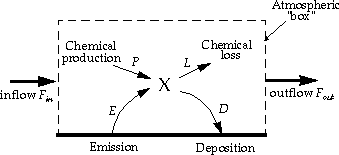
\includegraphics{Figures/boxmodel.png}
      \caption{ Standard box model parameters, image taken from \citet{Jacob_1999_book}. }
      \label{ch1:fig:boxmodel}
    \end{figure}

    
  \subsection{GEOS-Chem}
  
    GEOS-Chem is a well supported global, Eulerian CTM with a state of the science chemical mechanism, with transport driven by meteorological input from the Goddard Earth Observing System (GEOS) of the NASA Global Modeling and Assimilation Office (GMAO).
    GEOS-Chem simulates more than 100 chemical species from the earth's surface up to the edge of space (0.01 hPa) and can be used in combination with remote and in-situ sensing data to give a verifiable estimate of atmospheric gases and aerosols.
    It was developed, and is maintained, by Harvard University staff as well as users and researchers worldwide. 
    Several driving meteorological fields exist with different resolutions, the finest at 0.25 by 0.3125$^\circ$ horizontally at 5 minute time steps with 72 vertical levels.

    Combining satellite data with model outcomes provides a platform for the understanding of natural processes to be tested now and into the future over Australia and anywhere with few in-situ measurements.
    Due to the low availability of in-situ data covering most of the Australian continent, a combination of the models with satellite data may provide improved understanding of emissions from Australian landscapes.
    Improved emissions estimates will in turn improve the accuracy of CTMs, providing better predictions of atmospheric composition and its response to ongoing environmental change.

%----------------------------------------------------------------------------------------
%	SECTION 7
%----------------------------------------------------------------------------------------
\section{Satellites}
\label{ch1:sec:satellites}

  \subsection{Useful satellites}
    Several satellites provide long term trace gas observations with near complete global coverage, including the ERS-2 launched in April 1995 which houses the GOME ultraviolet and visible (UV-Vis) spectrometer, the AURA launched in July 2004 which houses the OMI UV-Vis spectrometer, the MetOp-A and B launched in October 2006 and September 2012 respectively both housing a GOME-2 UV-Vis spectrometer.
    These satellites are on Low Earth Orbit (LEO) trajectories and overpass any area up to once per day. 
    They record near nadir (nearly vertical) reflected spectra between around 250-700~nm split into spectral components at around $0.3$~nm in order to calculate trace gases including O$_3$, NO$_2$, and HCHO.
    An example of a spectrum retrieved from the GOME-2 instrument is given in figure \ref{ch1:fig:gomeproducts}.

    \begin{figure}
      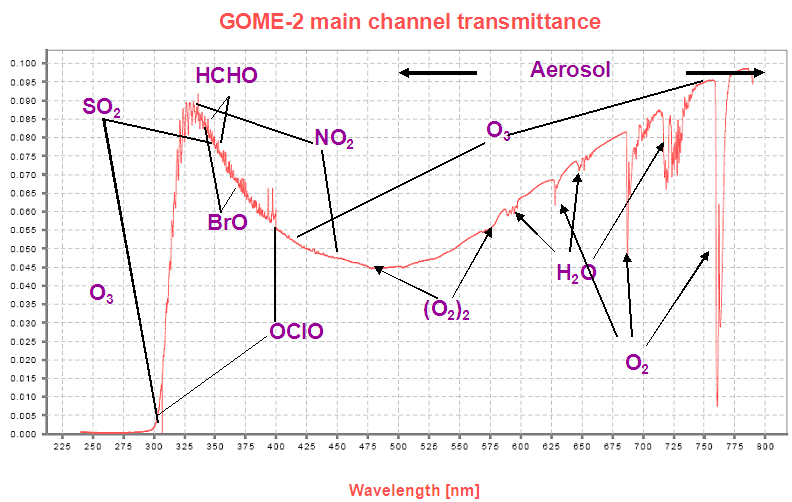
\includegraphics[width=\textwidth]{Figures/GOME_SPECTRUM.jpg}
      \caption{An example spectrum showing interferences used for species concentration measurements by GOME-2. Image by EUMETSAT and ESA \citep{GOME2Image}.}
      \label{ch1:fig:gomeproducts}
    \end{figure}

    
    Formaldehyde (HCHO) is often used as a proxy to estimate isoprene emissions \citep{Marais_2012,bauwens2013satellite}.
    Satellites can use DOAS techniques with radiative transfer calculations on solar radiation absorption spectra to measure column HCHO (eg: \citet{Leue_2001}).
    Several public data servers are available which include products from the satellites just mentioned, including NASA's Mirador (http://mirador.gsfc.nasa.gov/) and the Belgian Institute for Space Aeronomy (IASB-BIRA) Aeronomie site (http://h2co.aeronomie.be/).

    Instruments including MODIS on board the AQUA and TERRA satellites are able to determine aerosol optical depth (AOD), a measure of atmospheric scatter and absorbance. 
    An AOD of under 0.05 indicates a clear sky, while values of 1 or greater indicate increasingly hazy conditions.
    This is an important atmospheric property allowing us to track dust storms and pollution events as well as determine where measurements from other instruments may be compromised by high AOD.
    Satellite measured AOD requires validation by more accurate ground based instruments like those of AERONET which uses more than 200 sun photometers scattered globally. 
  
  \subsection{Comparisons with Models}
  
    DOAS methods can be heavily influenced by the initial estimates of a trace gas profile (the a priori) which is often produced by modelling, so when comparing models of these trace gases to satellite measurements extra care needs to be taken to avoid introducing bias from unrealistic a priori assumptions.
    A way to remove these a priori influences in order to compare models and satellites is through the satellite's averaging kernal, which is a measure of the sensitivity of the instrument to the trace gas's radiance at various heights multiplied by the sensitivity of the DOAS technique's forward radiative transfer model (RTM) to the amount of trace gas at various heights near the a priori \citep{Eskes_2003}.
  
  \subsection{DOAS}
    TODO: some of this is repeated in isoprene chapter satellite section.
    
    The DOAS technique uses solar radiation absorption spectra to measure trace gases through paths of light.
    The RTM used in DOAS techniques is based on Beer's law relating the attenuation of light to the properties of the medium it travels through.
    Beer's law states that $ T = I/I_0 = e^{-\tau} $ with T being transmittance, $\tau$ being optical depth, and I, I$_0$ being radiant flux received at instrument and emitted at source respectively.
    Using 
    $ \tau_i = \int \rho_i \beta_i ds $ gives us:
    $$ I = I_0 \exp {\left( \Sigma_i \int \rho_i \beta_i ds \right) } $$
    Where i represents a chemical species index, $\rho$ is a species density(molecules per cm$^3$), $\beta$ is the scattering and absorption cross section area (cm$^2$), and the integral over ds represents integration over the path from light source to instrument.
    The forward RTM used for satellite data products also involves functions representing extinction from Mie and Rayleigh scattering, and the efficiency of these on intensities from the trace gas under inspection, as well as accounting for various atmospheric parameters which may or may not be estimated (e.g. albedo).
    
    To convert the trace gas profile from a reflected solar radiance column (slanted along the light path) into a purely vertical column requires calculations of an air mass factor (AMF).
    In satellite data, the AMF is typically a scalar value for each horizontal grid point which will equal the ratio of the total vertical column density to the total slant column density. This value should also account for instrument sensitivities to various wavelengths at various altitudes, and is unique for each trace gas under consideration.
  